%\title{Creating an index with the makeidx package}
% Example from http://www.dickimaw-books.com/latex/thesis/html/makeidx.html

\documentclass[12pt,oneside]{scrbook} 

\usepackage{makeidx} 
\usepackage{minted}
\usepackage[french]{babel}
\usepackage{graphicx}
\selectlanguage{french}
\usepackage[T1]{fontenc}
\usepackage[utf8]{inputenc}
\usepackage{xcolor}
\usepackage{caption} 
\definecolor{bg}{rgb}{0.95,0.95,0.95}
\definecolor{bg_js}{rgb}{0.95,0.55,0.55}
\newminted{typescript}{javascript,bgcolor=bg}

\makeindex 

\title{Electron} 
\author{Me}
\date{\today}

\begin{document} 
\maketitle 
\tableofcontents


%\includegraphics{util_inherits.png}

%%%%%%%%%%%%%%NPM/Node
\chapter{Débuts}
\section{Installation}
Utilisation de NPM pour cela.
\begin{itemize}
\item Initialisation du projet
\begin{minted}[bgcolor=bg]{javascript}
npm init
\end{minted}
Le fichier package.json ressemble à ça:
\begin{minted}[bgcolor=bg]{shell}
{
  "name": "videoinfo",
  "version": "1.0.0",
  "description": "",
  "main": "index.js",
  "scripts": {
    "test": "echo \"Error: no test specified\" && exit 1"
  },
  "author": "",
  "license": "ISC",
  "dependencies": {
    "electron": "^1.7.6"
  }
}
\end{minted}
\item Ajout d'Electron\\
Dans ce projet vide, on ajoute la dépendance Elctron
\begin{minted}[bgcolor=bg]{shell}
npm install electron --save
\end{minted}

\end{itemize}
Et voilà, c'est intallé.

%%%%%%%%%%%%%%%
%%%% Premiers pas
\section{Premiers pas}
Les scripts commencent par l'inclusion d'electron:
\begin{minted}[bgcolor=bg]{javascript}
const electron = require('electron');
\end{minted}
On récupère l'objet \textit{app} de l'application electron qui vient d'être récupérée:
\begin{minted}[bgcolor=bg]{javascript}
const {app} = electron;
\end{minted}

\begin{minted}[bgcolor=bg]{javascript}
app.on('ready', ()=> {
    console.log('Hello world!!');
});
\end{minted}
Afin de pouvoir être exécuté, il faut pour cela indiquer comment il faut faire dans package.json dans la balise \textit{scripts}.
\begin{minted}[bgcolor=bg]{javascript}
"scripts": {
    "electron":"electron ."
  },
\end{minted}
Maintenant pour lancer l'application:
\begin{minted}[bgcolor=bg]{shell}
npm run electron
\end{minted}
Aucune fenêtre n'apparaît, mais dans les log on peut voir "Hello world" comme demandé dans le code. 
Pour afficher une fenêtre, il faut utilier l'objet \textit{BrowserWindows}
\begin{minted}[bgcolor=bg]{javascript}
//ajout de borwserWindow en définition
const {app, BrowserWindow} = electron;
app.on('ready', ()=> {
    new BrowserWindow({});
});
\end{minted}
Avec un objet vide en paramètre, il permet d'ouvrir une fenêtre vide, sans aucun affichage et avec un menu simple.

Pour avoir maintenant une page Web dans notre fenêtre, il faut maintenant créer un fichier .html
\begin{listing}[ht]
\begin{minted}[bgcolor=bg]{html}
<html>
<head>
</head>
<body>
    <h1>Titre</h1>
    <p>Pour l'instant une fenêtre vide.</p>
</body>
</html>
\end{minted}
\caption{fichier index.html}
\label{listing:0}
\end{listing}
Ensuite l'ouverture de ce fichier se fait comme suit:
\begin{minted}[bgcolor=bg]{javascript}
app.on('ready', ()=> {
    const mainWindow = new BrowserWindow({});
    mainWindow.loadURL(`file://${__dirname}/index.html`);
});
\end{minted}
A partir de cet instant, il n'est plus nécessaire de relancer l'application \textit{electron} pour voir un changement dans le fichier \textit{index.html} apparaître dans la fenêtre. Il suffit de recharger la page depuis le menu de la fenêtre.

\chapter{IPC}
Inter process communication permet de dialoguer entre la fenêtre HTML et NodeJS (electron). Cela se fait par le biai d'événement.
\section{Principe}
Electron a mis en place au sein du navigateur Chromium intégré des fonction permettant des communication IPC. Elles sont accéssible depuis une page HTML, mais pour pouvoir y accéder il faut préalablement utiliser la fonction \textit{require} comme dans un script NodeJS.

Il peut sembler étranger qu'une fonction require puisse exister directement dans la page HTML car normalement elle n'existe pas.

\begin{center}
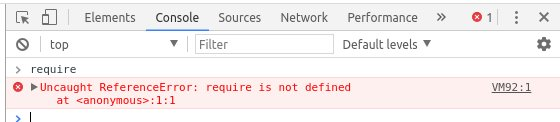
\includegraphics[width=\textwidth]{./img/chrome_require_fail.jpg}
\captionof{figure}{Fonction \textit{require} inconnue dans Chromium}
\label{fig1}
\end{center}

Si on effectue la même commande dans le console de la fenêtre d'electron (une fois activé les outils de débuggage), on remarque cette fois que la fonction existe:

\begin{center}
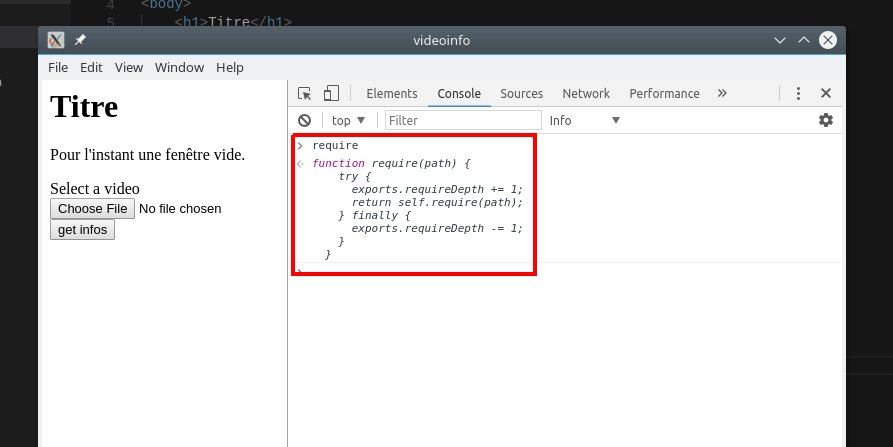
\includegraphics[width=\textwidth]{./img/chrome_require_ok.jpg}
\captionof{figure}{Fonction \textit{require} connue dans Electron}
\label{fig1}
\end{center}

Cela est dû au fait que dans Electron, la fenêtre qui apparaît contient déjà un ensemble de fonctionnalités que ne possède pas un navigateur classique.

\begin{center}
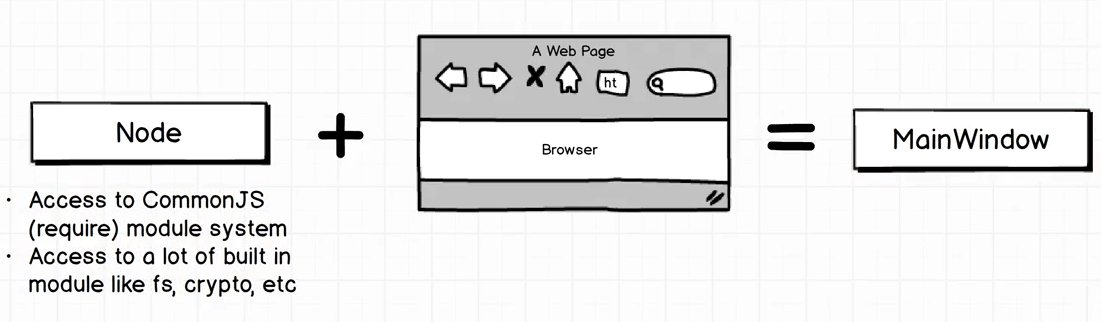
\includegraphics[width=\textwidth]{./img/electron_ajout.jpg}
\captionof{figure}{La fenêtre (MainWindow) est un condensé de fonctionnalités héritées de NodeJS avec le fonctionnement standard d'une page Web}
\label{fig1}
\end{center}

Cela permet d'accéder directement depuis la page Electron a des fonction IPC, et même aux fonctionnalités d'accès aux fichier:
\begin{minted}[bgcolor=bg]{javascript}
const fs = require('fs'); //<---- ceci fonctionne nativement
\end{minted}

\section{Exemple simple}





%%%%%%%%%%%%%%%
%%%%%%%%%ANNXES

\chapter{Annexes}
\section{Truc et astuces}
\subsection{Rafraîchir la page}
A partir du moment où une page apparaît dans la fenêtre, si une modification survient et que celle-ci n'a aucun lien avec la partie Javscript du côté electron, alors il n'est pas nécessaire de relancer electron.

En effet, il s'agit d'une page purement HTML avec son propre code Javascript, elle peut être rafraîchie/rechargée sans qu'il n'y ait d'impact avec le code NodeJS. \textbf{En revanche}, il peut y avoir des impacts en cas d'appel de formulaire ou de perte de données stockées temporairement en mémoire.
\subsection{Débuggage d'un événement}
On peut forcer directement depuis le code javascript un arrêt par le debugger. Si on est dans une fonction, ou un événement et que l'on souhaite s'arrêter dedans sans avoir à replacer le berakpoint depuis l'interface de debuggage, on ajoute une commande directement dans le code.
\begin{minted}[bgcolor=bg]{javascript}
document.querySelector('form').addEventListener('submit', 
    (event)=>{
        //pour pas que le formulaire se soumette tout seul
      event.preventDefault();  
      debugger      //<------- ICI
    })
\end{minted}
Pour que l'arrêt se produise, il faut activer le mode debuggage de la fenêtre. Dans le cas contraire, il ne va rien se produire.
\backmatter 

\printindex 

\end{document} 